% Edit only the text between matching begin and end lines.
\documentclass[11pt,a4paper]{article}
% Shared preamble for TMUA question papers. Local edits here are overwritten.

% Reproducible PDFs: no timestamps, no trailer id, no build-path details.
\ifdefined\pdfsuppressptexinfo
  \pdfsuppressptexinfo=-1
  \pdfinfoomitdate=1
  \pdftrailerid{}
\fi

\usepackage{graphicx}
\usepackage{mathtools}
\usepackage{amssymb}
\usepackage{amsmath}
\usepackage{amsthm}
\usepackage{enumitem}
\usepackage{microtype}
\usepackage[table]{xcolor}
\usepackage{array}
\usepackage{booktabs}
\usepackage{tabularx}
\usepackage{longtable}
\usepackage{ragged2e}
\usepackage{fancyhdr}
\usepackage{etoolbox}
\usepackage[
  a4paper,
  left=0.8in,
  right=1in,
  top=1in,
  bottom=0.5in,
  headheight=14pt,
  headsep=0.4in
]{geometry}

\usepackage{pgfplots}
\pgfplotsset{compat=1.18}
\usepgfplotslibrary{fillbetween, polar}
\usetikzlibrary{calc, positioning}
\usetikzlibrary{angles, quotes}
\usetikzlibrary{arrows.meta}
\usetikzlibrary{decorations.pathreplacing, decorations.markings}
\usetikzlibrary{patterns}
\usetikzlibrary{intersections}

\usepackage{tocloft}
\usepackage[hidelinks]{hyperref}
\hypersetup{pdfauthor={danieljsmith.org}, pdfcreator={}, pdfsubject={}, pdfkeywords={}}
\urlstyle{same}
\tocloftpagestyle{djspaper}
\setlength{\cftbeforesubsecskip}{2pt}
\setlength{\cftsubsecindent}{1.5em}
\setlength{\cftsubsecnumwidth}{0pt}
\renewcommand{\cftsubsecfont}{\small\color{black}}
\renewcommand{\cftsubsecpagefont}{\small\color{black}}
\renewcommand{\cftsubsecleader}{\hfill}

% \djsPaperSetup{<PDF title>}{<header label>}, called once after this file.
\newcommand{\djsHeaderLabel}{}
\newcommand{\djsPaperSetup}[2]{%
  \hypersetup{pdftitle={#1}}%
  \renewcommand{\djsHeaderLabel}{#2}}

\setlength{\parindent}{0pt}
\fancypagestyle{djspaper}{%
  \fancyhead{}%
  \fancyfoot{}%
  \renewcommand{\headrulewidth}{0.9pt}%
  \fancyhead[L]{\djsHeaderLabel}%
  \fancyhead[R]{\href{https://danieljsmith.org}{danieljsmith.org}}%
}
\pagestyle{djspaper}

\newcolumntype{Y}{>{\RaggedRight\arraybackslash}X}

% Topic labels: a subtle line above each question and a suffix on its
% contents entry. The bookmark form is spelled out separately, because a PDF
% bookmark is plain text and would otherwise keep the colour name.
\newcommand{\djsTocTopic}[1]{%
  \ifblank{#1}{}{%
    \texorpdfstring
      {\hspace{0.9em}{\footnotesize\itshape\color{black!45}#1}}
      { \textendash\ #1}}}
\newcommand{\djsTopicLine}[1]{%
  \ifblank{#1}{}{%
    {\raggedleft\footnotesize\itshape\color{black!45}#1\par}%
    \vspace{-0.6\baselineskip}}}

\newcommand{\questionitem}[1][]{%
  \item\phantomsection
  \addcontentsline{toc}{subsection}{%
    Question \number\value{enumi}\protect\djsTocTopic{#1}}%
}
\renewcommand{\contentsname}{Questions}
\newcommand{\djsFrontMatter}{%
  \vspace*{20pt}%
  \tableofcontents
  \newpage
}

\djsPaperSetup{TMUA Set A Paper 2}{TMUA Set A - Paper 2}
\begin{document}
\thispagestyle{djspaper}
\djsFrontMatter
\thispagestyle{djspaper}
\vspace*{8pt}
\djsTopicLine{Proof \& Error Analysis}
\begin{enumerate}[label=\textbf{\arabic*.},leftmargin=*,itemsep=0pt,start=1]
\questionitem[Proof \& Error Analysis]
% begin q000646 stem

Let $x$ and $y$ be real numbers.

A student attempts to prove the following claim: \begin{center}
\begin{minipage}{0.82\linewidth}
\centering
\textbf{Claim:} If $x+y\geq2$ then $x^2+y^2\ge 2$
\end{minipage}
\end{center} The student's attempt is as follows:

\[
\begin{array}{@{}rl@{}}
\textbf{Line 1:} &
\text{Since }x+y\ge2,\text{ at least one of }x\text{ and }y\text{ is at least }1. \\[-1pt]
&
\text{Assume }x\ge1;\text{ the other case is the same with }x\text{ and }y\text{ swapped.} \\[5pt]

\textbf{Line 2:} &
\text{From }x+y\ge2\text{ we get }y\ge2-x \\[5pt]

\textbf{Line 3:} &
\text{Therefore }y^2\ge(2-x)^2 \\[5pt]

\textbf{Line 4:} &
\text{Hence }x^2+y^2\ge x^2+(2-x)^2 \\[5pt]

\textbf{Line 5:} &
\text{Now }x^2+(2-x)^2=2(x-1)^2+2,\text{ and this is at least }2. \\[5pt]

\textbf{Line 6:} &
\text{Therefore }x^2+y^2\ge2,\text{ as claimed.}\\[5pt]
\end{array}
\]


Which of the following best describes the argument?
% end q000646 stem

\par\vspace*{12pt}
\begin{tabularx}{\linewidth}{@{}>{\bfseries}l Y@{}}
A &
% begin q000646 choice A
Line 1 contains the first error.
% end q000646 choice A
\\[0.8em]
B &
% begin q000646 choice B
Line 2 contains the first error.
% end q000646 choice B
\\[0.8em]
C &
% begin q000646 choice C
Line 3 contains the first error.
% end q000646 choice C
\\[0.8em]
D &
% begin q000646 choice D
Line 4 contains the first error.
% end q000646 choice D
\\[0.8em]
E &
% begin q000646 choice E
Line 5 contains the first error.
% end q000646 choice E
\\[0.8em]
F &
% begin q000646 choice F
The argument is a correct proof of the claim.
% end q000646 choice F
\\[0.8em]
G &
% begin q000646 choice G
The argument contains no error, but the claim is false.
% end q000646 choice G
\\
\end{tabularx}
\end{enumerate}
\clearpage
\thispagestyle{djspaper}
\vspace*{8pt}
\djsTopicLine{Trigonometry}
\begin{enumerate}[label=\textbf{\arabic*.},leftmargin=*,itemsep=0pt,start=2]
\questionitem[Trigonometry]
% begin q000636 stem
In quadrilateral $ABCD$, the diagonal $AC$ divides the figure into two right-angled triangles, $\triangle ABC$ and $\triangle ACD$.

\begin{itemize}
    \item In $\triangle ABC$, $\angle ABC = 90^\circ$, $\angle BAC = 30^\circ$, and $AB = \sqrt{6}\text{ cm}$
    \item In $\triangle ACD$, $\angle ACD = 90^\circ$, and $\tan(\angle CAD) = \dfrac{1}{\sqrt{2}}$
\end{itemize}

What is the area of quadrilateral $ABCD$, in $\text{cm}^2$? \\
% end q000636 stem

\par\vspace*{12pt}
\begin{tabularx}{\linewidth}{@{}>{\bfseries}l Y@{}}
A &
% begin q000636 choice A
$\sqrt{3} + \sqrt{2}$
% end q000636 choice A
\\[0.8em]
B &
% begin q000636 choice B
$\sqrt{3} + 2\sqrt{2}$
% end q000636 choice B
\\[0.8em]
C &
% begin q000636 choice C
$2\sqrt{3} + \sqrt{2}$
% end q000636 choice C
\\[0.8em]
D &
% begin q000636 choice D
$2\sqrt{3} + 2\sqrt{2}$
% end q000636 choice D
\\[0.8em]
E &
% begin q000636 choice E
$\sqrt{3} + 4\sqrt{2}$
% end q000636 choice E
\\[0.8em]
F &
% begin q000636 choice F
$2\sqrt{3} + 4\sqrt{2}$
% end q000636 choice F
\\
\end{tabularx}
\end{enumerate}
\clearpage
\thispagestyle{djspaper}
\vspace*{8pt}
\djsTopicLine{Proof \& Error Analysis}
\begin{enumerate}[label=\textbf{\arabic*.},leftmargin=*,itemsep=0pt,start=3]
\questionitem[Proof \& Error Analysis]
% begin q000681 stem
Consider the following claim and attempted proof.

\begin{center}
\begin{minipage}{0.82\linewidth}
\centering
\textbf{Claim:} Let $f(x)$ be a quadratic polynomial. If $\displaystyle\int_{-1}^{1} f(x)\,\mathrm{d}x = 0$, then the graph of $y = f(x)$ must intersect the $x$-axis at two distinct points in the interval $-1 < x < 1$.
\end{minipage}
\end{center}
Attempted proof:
\[
\begin{array}{@{}rl@{}}
\textbf{Line 1} & \text{Let } f(x) = ax^2 + bx + c\text{, where } a, b, c \text{ are real constants with } a \ne 0 \\[5pt]
\textbf{Line 2} & \text{Evaluating the integral gives } \displaystyle\int_{-1}^{1} f(x)\,\mathrm{d}x = \frac{2a}{3} + 2c = 0\text{, so } c = -\frac{a}{3} \\[12pt]
\textbf{Line 3} & \text{The roots } x_1 \text{ and } x_2 \text{ of } f(x) = 0 \text{ satisfy } x_1 x_2 = \frac{c}{a} = -\frac{1}{3} \\[7pt]
\textbf{Line 4} & \text{Since } x_1 x_2 < 0\text{, the discriminant } b^2 - 4ac = b^2 + \frac{4a^2}{3} > 0\\ & \text{so the roots are real and distinct} \\[7pt]
\textbf{Line 5} & \text{Since } |x_1 x_2| = \frac{1}{3} < 1\text{, it follows that } |x_1| < 1 \text{ and } |x_2| < 1 \\[7pt]
\textbf{Line 6} & \text{Therefore, both roots lie in the interval } -1 < x < 1\\[5pt]
\end{array}
\]

Which line of the proof contains the first error?
% end q000681 stem

\par\vspace*{12pt}
\begin{tabularx}{\linewidth}{@{}>{\bfseries}l Y@{}}
A &
% begin q000681 choice A
Line 1
% end q000681 choice A
\\[0.8em]
B &
% begin q000681 choice B
Line 2
% end q000681 choice B
\\[0.8em]
C &
% begin q000681 choice C
Line 3
% end q000681 choice C
\\[0.8em]
D &
% begin q000681 choice D
Line 4
% end q000681 choice D
\\[0.8em]
E &
% begin q000681 choice E
Line 5
% end q000681 choice E
\\[0.8em]
F &
% begin q000681 choice F
Line 6
% end q000681 choice F
\\[0.8em]
G &
% begin q000681 choice G
There is no error, the proof is correct as written.
% end q000681 choice G
\\
\end{tabularx}
\end{enumerate}
\clearpage
\thispagestyle{djspaper}
\vspace*{8pt}
\djsTopicLine{Exponentials \& Logarithms}
\begin{enumerate}[label=\textbf{\arabic*.},leftmargin=*,itemsep=0pt,start=4]
\questionitem[Exponentials \& Logarithms]
% begin q000046 stem
Let $a$ be a positive real number with $a \ne 1$

The equation \[ \log_a(3x-1) = 2 + \log_a(x+1) \] has exactly one real solution $x$

What is the complete range of all the possible values of $a$?
% end q000046 stem

\par\vspace*{12pt}
\begin{tabularx}{\linewidth}{@{}>{\bfseries}l Y@{}}
A &
% begin q000046 choice A
$0<a<\sqrt{3}$ and $a\ne 1$
% end q000046 choice A
\\[0.8em]
B &
% begin q000046 choice B
$a > 1$
% end q000046 choice B
\\[0.8em]
C &
% begin q000046 choice C
$a>0$ and $a \ne 1$
% end q000046 choice C
\\[0.8em]
D &
% begin q000046 choice D
No such $a$ exists
% end q000046 choice D
\\[0.8em]
E &
% begin q000046 choice E
$a=3$
% end q000046 choice E
\\[0.8em]
F &
% begin q000046 choice F
$a=\frac{1}{3}$
% end q000046 choice F
\\[0.8em]
G &
% begin q000046 choice G
$a>0$, $a \ne 1$ and $a \ne \sqrt{3}$
% end q000046 choice G
\\
\end{tabularx}
\end{enumerate}
\clearpage
\thispagestyle{djspaper}
\vspace*{8pt}
\djsTopicLine{Number}
\begin{enumerate}[label=\textbf{\arabic*.},leftmargin=*,itemsep=0pt,start=5]
\questionitem[Number]
% begin q000592 stem
A positive integer $n$ can be written as $n = 2^a3^b$ where $a$ and $b$ are non-negative integers. 

The number $n$ has exactly $12$ positive factors, counting $1$ and $n$ itself. 

Given that $n<200$, what is the greatest possible value of $n$?
% end q000592 stem

\par\vspace*{12pt}
\begin{tabularx}{\linewidth}{@{}>{\bfseries}l Y@{}}
A &
% begin q000592 choice A
$72$
% end q000592 choice A
\\[0.8em]
B &
% begin q000592 choice B
$96$
% end q000592 choice B
\\[0.8em]
C &
% begin q000592 choice C
$108$
% end q000592 choice C
\\[0.8em]
D &
% begin q000592 choice D
$144$
% end q000592 choice D
\\[0.8em]
E &
% begin q000592 choice E
$162$
% end q000592 choice E
\\[0.8em]
F &
% begin q000592 choice F
$486$
% end q000592 choice F
\\
\end{tabularx}
\end{enumerate}
\clearpage
\thispagestyle{djspaper}
\vspace*{8pt}
\djsTopicLine{Proof \& Error Analysis}
\begin{enumerate}[label=\textbf{\arabic*.},leftmargin=*,itemsep=0pt,start=6]
\questionitem[Proof \& Error Analysis]
% begin q000648 stem
Let $a$ and $b$ be real numbers. A student attempts to prove the following claim: 
\begin{center} \begin{minipage}{0.82\linewidth} \centering \textbf{Claim:} If $a+b$ and $ab$ are both integers, then $a$ and $b$ are both integers. \end{minipage} \end{center}

The student's attempt is as follows:\[
\begin{array}{@{}rl@{}}
\textbf{I} &
\text{$a$ and $b$ are the two solutions of }
t^2-(a+b)t+ab=0 \\[10pt]

\textbf{II} &
\text{Write }s=a+b\text{ and }p=ab,\text{ so }s\text{ and }p\text{ are integers and} \\[-1pt]
&
\displaystyle
\text{the two solutions are }
t=\frac{s\pm\sqrt{s^2-4p}}{2} \\[10pt]

\textbf{III} &
\text{Since }a\text{ and }b\text{ are real, }s^2-4p\geq0 \\[10pt]

\textbf{IV} &
\text{Also }s^2-4p\text{ is an integer, so }\sqrt{s^2-4p}
\text{ is either an integer or an irrational number.} \\[10pt]

\textbf{V} &
\text{If }\sqrt{s^2-4p}\text{ were irrational, then }a\text{ would be irrational,} \\[-1pt]
&
\text{and so }a+b\text{ would be irrational, contradicting the fact that }
a+b\text{ is an integer.} \\[10pt]

\textbf{VI} &
\text{Hence }\sqrt{s^2-4p}\text{ is an integer, so }
s\pm\sqrt{s^2-4p}\text{ is an integer,} \\[-1pt]
&
\text{and therefore }a\text{ and }b\text{ are both integers.}
\end{array}
\]

Which of the following best describes this attempt?
% end q000648 stem

\par\vspace*{12pt}
\begin{tabularx}{\linewidth}{@{}>{\bfseries}l Y@{}}
A &
% begin q000648 choice A
It is completely correct.
% end q000648 choice A
\\[0.8em]
B &
% begin q000648 choice B
It is incorrect, and the first error is on line I.
% end q000648 choice B
\\[0.8em]
C &
% begin q000648 choice C
It is incorrect, and the first error is on line II.
% end q000648 choice C
\\[0.8em]
D &
% begin q000648 choice D
It is incorrect, and the first error is on line III.
% end q000648 choice D
\\[0.8em]
E &
% begin q000648 choice E
It is incorrect, and the first error is on line IV.
% end q000648 choice E
\\[0.8em]
F &
% begin q000648 choice F
It is incorrect, and the first error is on line V.
% end q000648 choice F
\\[0.8em]
G &
% begin q000648 choice G
It is incorrect, and the first error is on line VI.
% end q000648 choice G
\\
\end{tabularx}
\end{enumerate}
\clearpage
\thispagestyle{djspaper}
\vspace*{8pt}
\djsTopicLine{Geometry}
\begin{enumerate}[label=\textbf{\arabic*.},leftmargin=*,itemsep=0pt,start=7]
\questionitem[Geometry]
% begin q000569 stem
Triangle $ABC$ is right-angled at $A$, with $AB=6\,\mathrm{cm}$ and $AC=8\,\mathrm{cm}$.

Semicircles are drawn with $AB$, $AC$ and $BC$ as diameters, as shown. The semicircle on $BC$ is on the same side of the line $BC$ as $A$. The portions of the other two semicircles that lie outside the semicircle on $BC$ are shaded.

What is the total shaded area, in $\mathrm{cm}^2$?
% end q000569 stem

\begin{center}
% begin q000569 diagram
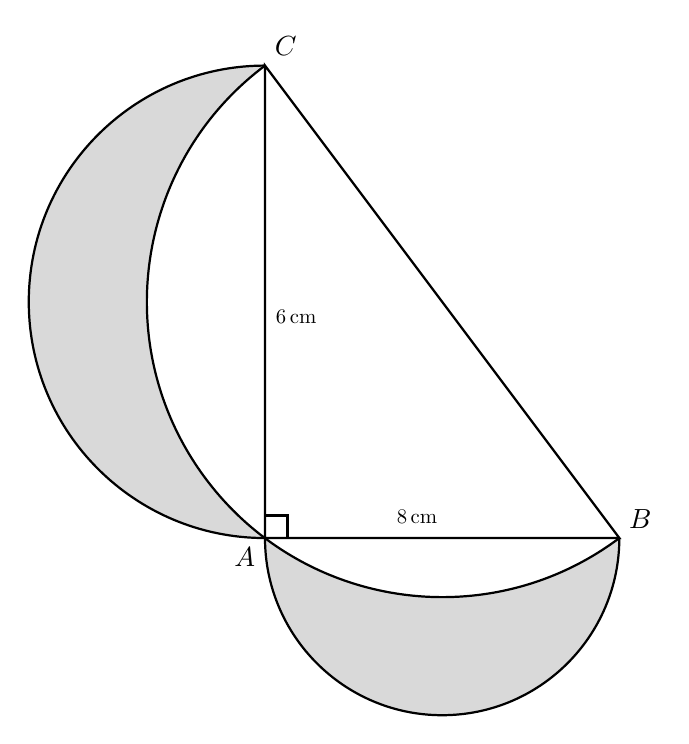
\begin{tikzpicture}[scale=0.75]
\def\AB{6}
\def\AC{8}
\def\ra{0.38}
\pgfmathsetmacro{\rAB}{\AB/2}
\pgfmathsetmacro{\rAC}{\AC/2}
\pgfmathsetmacro{\rBC}{sqrt(\AB*\AB+\AC*\AC)/2}
\pgfmathsetmacro{\alphaang}{atan(\AC/\AB)}
\pgfmathsetmacro{\angB}{-\alphaang}
\pgfmathsetmacro{\angA}{\alphaang-180}
\pgfmathsetmacro{\angC}{-\alphaang-180}

\coordinate (A) at (0,0);
\coordinate (B) at (\AB,0);
\coordinate (C) at (0,\AC);

% Shaded lune adjacent to AB
\path[fill=gray!30]
  (A) arc[start angle=180,end angle=360,radius=\rAB]
  arc[start angle=\angB,end angle=\angA,radius=\rBC]
  -- cycle;

% Shaded lune adjacent to AC
\path[fill=gray!30]
  (A) arc[start angle=-90,end angle=-270,radius=\rAC]
  arc[start angle=\angC,end angle=\angA,radius=\rBC]
  -- cycle;

% Three semicircular arcs
\draw[thick, black] (A) arc[start angle=180,end angle=360,radius=\rAB];
\draw[thick, black] (A) arc[start angle=-90,end angle=-270,radius=\rAC];
\draw[thick, black] (B) arc[start angle=\angB,end angle=\angC,radius=\rBC];

% Triangle and its diameters
\draw[thick, black] (A) -- (B) -- (C) -- cycle;

% Right-angle marker
\coordinate (RAx) at ($(A)+(\ra,0)$);
\coordinate (RAxy) at ($(A)+(\ra,\ra)$);
\coordinate (RAy) at ($(A)+(0,\ra)$);
\draw[thick] (RAx) -- (RAxy) -- (RAy);

% Labels
\node[below left] at (A) {$A$};
\node[above right] at (B) {$B$};
\node[above right] at (C) {$C$};
\node[midway, above, yshift=100pt, xshift=15pt] at ($(A)!0.5!(B)$) {$6\,\mathrm{cm}$};
\node[midway, right, yshift=10pt, xshift=60pt] at ($(A)!0.5!(C)$) {$8\,\mathrm{cm}$};
\end{tikzpicture}
% end q000569 diagram
\end{center}

\par\vspace*{12pt}
\begin{tabularx}{\linewidth}{@{}>{\bfseries}l Y@{}}
A &
% begin q000569 choice A
$12$
% end q000569 choice A
\\[0.8em]
B &
% begin q000569 choice B
$24$
% end q000569 choice B
\\[0.8em]
C &
% begin q000569 choice C
$30$
% end q000569 choice C
\\[0.8em]
D &
% begin q000569 choice D
$40$
% end q000569 choice D
\\[0.8em]
E &
% begin q000569 choice E
$48$
% end q000569 choice E
\\[0.8em]
F &
% begin q000569 choice F
$50$
% end q000569 choice F
\\
\end{tabularx}
\end{enumerate}
\clearpage
\thispagestyle{djspaper}
\vspace*{8pt}
\djsTopicLine{Coordinate Geometry}
\begin{enumerate}[label=\textbf{\arabic*.},leftmargin=*,itemsep=0pt,start=8]
\questionitem[Coordinate Geometry]
% begin q000629 stem
The line $y=3x+2$ meets the parabola $y=x^2$ at the points $P$ and $Q$. The tangents to the parabola at $P$ and $Q$ meet at $R$, as shown.

What are the coordinates of $R$?
% end q000629 stem

\begin{center}
% begin q000629 diagram
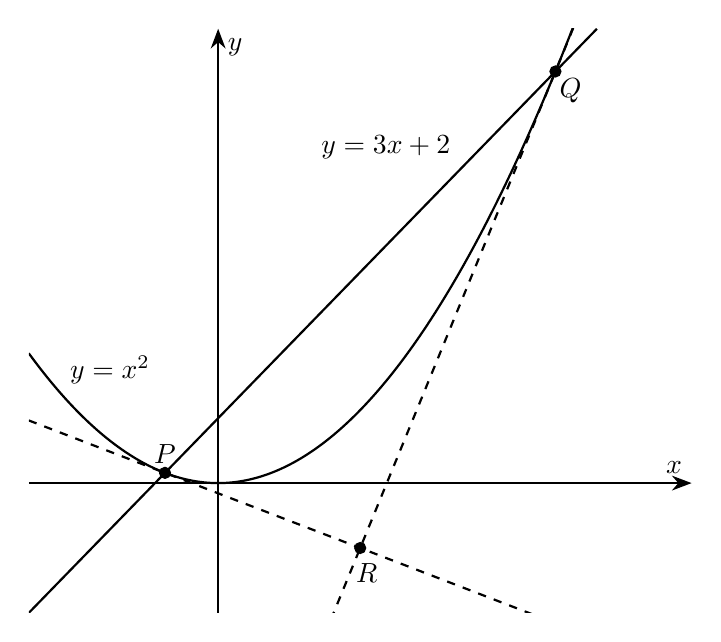
\begin{tikzpicture}
\pgfmathsetmacro{\px}{(3-sqrt(17))/2}
\pgfmathsetmacro{\qx}{(3+sqrt(17))/2}
\pgfmathsetmacro{\py}{(\px)*(\px)}
\pgfmathsetmacro{\qy}{(\qx)*(\qx)}
\pgfmathsetmacro{\rx}{(\px+\qx)/2}
\pgfmathsetmacro{\ry}{\px*\qx}

\pgfmathsetmacro{\curveLabelX}{-1.55}
\pgfmathsetmacro{\curveLabelY}{(\curveLabelX)*(\curveLabelX)}

\begin{axis}[
    width=10cm,
    height=9cm,
    axis lines=middle,
    axis line style={thick, black, -{Stealth[length=2.5mm]}},
    xlabel={$x$},
    ylabel={$y$},
    xmin=-2, xmax=5,
    ymin=-4, ymax=14,
    xtick=\empty,
    ytick=\empty,
    xticklabel=\empty,
    yticklabel=\empty,
    tick align=outside,
    enlargelimits=false,
    clip=true,
    samples=160
]

\coordinate (P) at (axis cs:\px,\py);
\coordinate (Q) at (axis cs:\qx,\qy);
\coordinate (R) at (axis cs:\rx,\ry);
\coordinate (curveLabel) at
    (axis cs:\curveLabelX,\curveLabelY);

% Parabola and secant
\addplot[thick, black, domain=-2:4, mark=none]
    {x^2};

\addplot[thick, black, domain=-2:4, samples=2, mark=none]
    {3*x+2}
    node[pos=0.76, above left] {$y=3x+2$};

% Tangents at P and Q
\addplot[dashed, black, thick, domain=-2:5, samples=2, mark=none]
    {2*(\px)*x-\py};

\addplot[dashed, black, thick, domain=-2:5, samples=2, mark=none]
    {2*(\qx)*x-\qy};

% Curve label
\node[above right, xshift=-4pt, yshift=4pt]
    at (curveLabel) {$y=x^2$};

% Marked points
\addplot[only marks, mark=*, mark size=2pt, black]
    coordinates {
        ({\px},{\py})
        ({\qx},{\qy})
        ({\rx},{\ry})
    };

\node[above, yshift=0pt] at (P) {$P$};
\node[below right, xshift=-2pt, yshift=1pt] at (Q) {$Q$};
\node[below right, xshift=-5pt, yshift=-2pt] at (R) {$R$};

\end{axis}
\end{tikzpicture}
% end q000629 diagram
\end{center}

\par\vspace*{12pt}
\begin{tabularx}{\linewidth}{@{}>{\bfseries}l Y@{}}
A &
% begin q000629 choice A
$\left(\dfrac{3}{2},-4\right)$
% end q000629 choice A
\\[0.8em]
B &
% begin q000629 choice B
$\left(\dfrac{3}{2},-2\right)$
% end q000629 choice B
\\[0.8em]
C &
% begin q000629 choice C
$\left(\dfrac{3}{2},-1\right)$
% end q000629 choice C
\\[0.8em]
D &
% begin q000629 choice D
$\left(3,-2\right)$
% end q000629 choice D
\\[0.8em]
E &
% begin q000629 choice E
$\left(1,-3\right)$
% end q000629 choice E
\\[0.8em]
F &
% begin q000629 choice F
$\left(2,-\dfrac{3}{2}\right)$
% end q000629 choice F
\\
\end{tabularx}
\end{enumerate}
\clearpage
\thispagestyle{djspaper}
\vspace*{8pt}
\djsTopicLine{Logic}
\begin{enumerate}[label=\textbf{\arabic*.},leftmargin=*,itemsep=0pt,start=9]
\questionitem[Logic]
% begin q000161 stem
Consider the statement:

\[ \begin{array}{c}
\text{\textbf{If} $0 \le f(x) \le 1$ for all real $x$ with $0 \le x \le 1$, \textbf{then}}\\[5pt]

\text{$\displaystyle\int_0^1 f(x)\,\mathrm{d}x \le \int_0^1 (f(x))^2\,\mathrm{d}x$} \\
\end{array} \tag{$\ast$} \] Which of the following functions is a \textit{counterexample} to ($\ast$)?
% end q000161 stem

\par\vspace*{12pt}
\begin{tabularx}{\linewidth}{@{}>{\bfseries}l Y@{}}
A &
% begin q000161 choice A
$f(x)=2x$
% end q000161 choice A
\\[0.8em]
B &
% begin q000161 choice B
$f(x)=x^2+\frac{1}{2}$
% end q000161 choice B
\\[0.8em]
C &
% begin q000161 choice C
$f(x)=\frac{1}{2}$
% end q000161 choice C
\\[0.8em]
D &
% begin q000161 choice D
$f(x)=1+x$
% end q000161 choice D
\\[0.8em]
E &
% begin q000161 choice E
$f(x)=0$
% end q000161 choice E
\\[0.8em]
F &
% begin q000161 choice F
$f(x)=5x(1-x)$
% end q000161 choice F
\\[0.8em]
G &
% begin q000161 choice G
$f(x)=\sqrt{x}+\frac{1}{2}$
% end q000161 choice G
\\[0.8em]
H &
% begin q000161 choice H
$f(x)=1$
% end q000161 choice H
\\
\end{tabularx}
\end{enumerate}
\clearpage
\thispagestyle{djspaper}
\vspace*{8pt}
\djsTopicLine{Logic}
\begin{enumerate}[label=\textbf{\arabic*.},leftmargin=*,itemsep=0pt,start=10]
\questionitem[Logic]
% begin q000687 stem
Consider the following three conditions on a positive real number $x$

\[
\begin{array}{@{}ll@{}}
(1) & x^2 - 3x + 2 < 0 \\[5pt]
(2) & \log_{10} x > 0 \\[5pt]
(3) & 2^x > 4 \\[5pt]
\end{array}\]

Which of the following statements is/are true?

\[
\begin{array}{@{}l l@{}}
\textbf{I:} & \text{Condition (2) holds only if at least one of conditions (1) and (3) holds} \\[8pt]
\textbf{II:} & \text{If condition (2) does not hold, then condition (3) does not hold} \\[8pt]
\textbf{III:} &
\begin{aligned}[t]
&\text{For condition (1) to hold, it is necessary but not sufficient} \\
&\text{that condition (3) does not hold} \\[5pt]
\end{aligned}
\end{array}
\]
% end q000687 stem

\par\vspace*{12pt}
\begin{tabularx}{\linewidth}{@{}>{\bfseries}l Y@{}}
A &
% begin q000687 choice A
None of them
% end q000687 choice A
\\[0.8em]
B &
% begin q000687 choice B
I only
% end q000687 choice B
\\[0.8em]
C &
% begin q000687 choice C
II only
% end q000687 choice C
\\[0.8em]
D &
% begin q000687 choice D
III only
% end q000687 choice D
\\[0.8em]
E &
% begin q000687 choice E
I and II only
% end q000687 choice E
\\[0.8em]
F &
% begin q000687 choice F
I and III only
% end q000687 choice F
\\[0.8em]
G &
% begin q000687 choice G
II and III only
% end q000687 choice G
\\[0.8em]
H &
% begin q000687 choice H
I, II and III
% end q000687 choice H
\\
\end{tabularx}
\end{enumerate}
\clearpage
\thispagestyle{djspaper}
\vspace*{8pt}
\djsTopicLine{Probability \& Counting}
\begin{enumerate}[label=\textbf{\arabic*.},leftmargin=*,itemsep=0pt,start=11]
\questionitem[Probability \& Counting]
% begin q000596 stem
A three-digit code is formed by selecting three different digits from $1,2,3,4,5,6$ and placing them in random order. 

Each possible code is equally likely.

It is revealed that the product of the three digits in the code is divisible by $6$.

What is the probability that the code contains the digit $6$?
% end q000596 stem

\par\vspace*{12pt}
\begin{tabularx}{\linewidth}{@{}>{\bfseries}l Y@{}}
A &
% begin q000596 choice A
$\dfrac{1}{3}$
% end q000596 choice A
\\[0.8em]
B &
% begin q000596 choice B
$\dfrac{1}{2}$
% end q000596 choice B
\\[0.8em]
C &
% begin q000596 choice C
$\dfrac{3}{5}$
% end q000596 choice C
\\[0.8em]
D &
% begin q000596 choice D
$\dfrac{2}{3}$
% end q000596 choice D
\\[0.8em]
E &
% begin q000596 choice E
$\dfrac{3}{4}$
% end q000596 choice E
\\[0.8em]
F &
% begin q000596 choice F
$\dfrac{5}{6}$
% end q000596 choice F
\\
\end{tabularx}
\end{enumerate}
\clearpage
\thispagestyle{djspaper}
\vspace*{8pt}
\djsTopicLine{Proof \& Error Analysis}
\begin{enumerate}[label=\textbf{\arabic*.},leftmargin=*,itemsep=0pt,start=12]
\questionitem[Proof \& Error Analysis]
% begin q000678 stem
Consider the claim about cubic polynomials: \\[-5pt]

\noindent\hbox to \linewidth{%
  \hfil
  \llap{\textbf{Claim:}\hspace{0.4em}}%
  \parbox[t]{0.7\linewidth}{\centering
    If a cubic polynomial $f$ has distinct roots $a$, $b$ and $c$, where $a<b<c$, then there exists $x$ with $a<x<b$ such that $f''(x)=0$}%
  \hfil} \\

The student attempts to prove the claim and produces the following argument:
\[
\begin{array}{@{}rl@{}}
\mathbf{I} & \text{Since } f(a)=f(b)=0,\text{ there is a number }p\text{ such that }a<p<b\text{ and }f'(p)=0 \\[5pt]
\mathbf{II} & \text{Similarly, there is a number }q\text{ such that }b<q<c\text{ and }f'(q)=0 \\[5pt]
\mathbf{III} & \text{The polynomial }f'\text{ is quadratic with roots }p\text{ and }q,\text{ so }f''\!\left(\frac{p+q}{2}\right)=0 \\[5pt]
\mathbf{IV} &
\text{Since }a<p<b<q<c,\text{ we have }p-b<0<q-b,\text{ and hence}\\[4pt]
&\displaystyle\qquad
\frac{p+q}{2}-b
=\frac{(p-b)+(q-b)}{2}<0 \\[5pt]
\mathbf{V} & \text{Therefore the claim is true, the claimed } x \text{ can be chosen as } x=\frac{p+q}{2}\\[5pt]
\end{array}
\]

Which line contains the first error?
% end q000678 stem

\par\vspace*{12pt}
\begin{tabularx}{\linewidth}{@{}>{\bfseries}l Y@{}}
A &
% begin q000678 choice A
Line $\mathbf{I}$
% end q000678 choice A
\\[0.8em]
B &
% begin q000678 choice B
Line $\mathbf{II}$
% end q000678 choice B
\\[0.8em]
C &
% begin q000678 choice C
Line $\mathbf{III}$
% end q000678 choice C
\\[0.8em]
D &
% begin q000678 choice D
Line $\mathbf{IV}$
% end q000678 choice D
\\[0.8em]
E &
% begin q000678 choice E
Line $\mathbf{V}$
% end q000678 choice E
\\[0.8em]
F &
% begin q000678 choice F
There is no error, the proof is correct as written.
% end q000678 choice F
\\
\end{tabularx}
\end{enumerate}
\clearpage
\thispagestyle{djspaper}
\vspace*{8pt}
\djsTopicLine{Integration}
\begin{enumerate}[label=\textbf{\arabic*.},leftmargin=*,itemsep=0pt,start=13]
\questionitem[Integration]
% begin q000120 stem
For each positive integer $n$, define \[ F(n)=\int_0^1 x^n\,\mathrm{d}x \] and \[ H(n)=\sum_{r=1}^n \frac{1}{F(r)} \]

What is the smallest positive integer $n$ such that $H(n)>15$?
% end q000120 stem

\par\vspace*{12pt}
\begin{tabularx}{\linewidth}{@{}>{\bfseries}l Y@{}}
A &
% begin q000120 choice A
$3$
% end q000120 choice A
\\[0.8em]
B &
% begin q000120 choice B
$4$
% end q000120 choice B
\\[0.8em]
C &
% begin q000120 choice C
$5$
% end q000120 choice C
\\[0.8em]
D &
% begin q000120 choice D
$6$
% end q000120 choice D
\\[0.8em]
E &
% begin q000120 choice E
$7$
% end q000120 choice E
\\
\end{tabularx}
\end{enumerate}
\clearpage
\thispagestyle{djspaper}
\vspace*{8pt}
\djsTopicLine{Logic}
\begin{enumerate}[label=\textbf{\arabic*.},leftmargin=*,itemsep=0pt,start=14]
\questionitem[Logic]
% begin q000125 stem
Let $S$ be the statement: \[ \begin{array}{c}
\text{For all real numbers $x$, if $|x| \ge 1$ then $g(x) > 0$}
\end{array} \] Which of the following is a correct \textbf{negation} of $S$?
% end q000125 stem

\par\vspace*{12pt}
\begin{tabularx}{\linewidth}{@{}>{\bfseries}l Y@{}}
A &
% begin q000125 choice A
There exists a real number $x$ with $|x| \ge 1$ such that $g(x) \le 0$
% end q000125 choice A
\\[0.8em]
B &
% begin q000125 choice B
There exists a real number $x$ with $|x| > 1$ such that $g(x) < 0$
% end q000125 choice B
\\[0.8em]
C &
% begin q000125 choice C
For all real numbers $x$, either $|x| < 1$ or $g(x) > 0$
% end q000125 choice C
\\[0.8em]
D &
% begin q000125 choice D
For all real numbers $x$ with $|x| \ge 1$, $g(x) \ge 0$
% end q000125 choice D
\\[0.8em]
E &
% begin q000125 choice E
There exists a real number $x$ such that $|x| < 1$ and $g(x) \le 0$
% end q000125 choice E
\\[0.8em]
F &
% begin q000125 choice F
There exists a real number $x$ such that $|x| < 1$ or $g(x) \le 0$
% end q000125 choice F
\\
\end{tabularx}
\end{enumerate}
\clearpage
\thispagestyle{djspaper}
\vspace*{8pt}
\djsTopicLine{Proof \& Error Analysis}
\begin{enumerate}[label=\textbf{\arabic*.},leftmargin=*,itemsep=0pt,start=15]
\questionitem[Proof \& Error Analysis]
% begin q000682 stem
A function $f$ is defined for all real $x$, and $f'(x)$ exists for every real $x$.

The function $f$ is also \textbf{strictly increasing:} whenever $a<b$, also $f(a)<f(b)$.

A student makes the following claim:
\begin{center}
\begin{minipage}{0.82\linewidth}
\centering
\textbf{Claim:} It follows that $f'(x)>0$ for every real $x$
\end{minipage}
\end{center}
The student argues as follows:

\[
\begin{array}{@{}rl@{}}
\textbf{Line 1:} & \text{Suppose, for a contradiction, that $f'(c)\le 0$ for some real number $c$} \\[5pt]
\textbf{Line 2:} & \text{If $f'(c)<0$, then just to the right of $c$ the graph of $f$ falls below} \\ 
& \text{$f(c)$, which contradicts $f$ being strictly increasing. Hence $f'(c)=0$} \\[5pt]
\textbf{Line 3:} & \text{So the tangent to the graph of $f$ at $x=c$ is horizontal} \\[5pt]
\textbf{Line 4:} & \text{A horizontal tangent at $x=c$ means there are numbers $a<c<b$ with} \\ 
& \text{$f(a)\ge f(c)$ or with $f(b)\le f(c)$} \\[5pt]
\textbf{Line 5:} & \text{Either possibility contradicts $f$ being strictly increasing. Hence} \\ 
& \text{$f'(x)>0$ for every real $x$} \\[5pt]
\end{array}
\]

Which of the following best describes the argument?
% end q000682 stem

\par\vspace*{12pt}
\begin{tabularx}{\linewidth}{@{}>{\bfseries}l Y@{}}
A &
% begin q000682 choice A
The argument is correct, and the claim is true
% end q000682 choice A
\\[0.8em]
B &
% begin q000682 choice B
The first error occurs in Line 2
% end q000682 choice B
\\[0.8em]
C &
% begin q000682 choice C
The first error occurs in Line 3
% end q000682 choice C
\\[0.8em]
D &
% begin q000682 choice D
The first error occurs in Line 4
% end q000682 choice D
\\[0.8em]
E &
% begin q000682 choice E
The first error occurs in Line 5
% end q000682 choice E
\\[0.8em]
F &
% begin q000682 choice F
The argument contains an error, but the claim is nevertheless true
% end q000682 choice F
\\
\end{tabularx}
\end{enumerate}
\clearpage
\thispagestyle{djspaper}
\vspace*{8pt}
\djsTopicLine{Sequences \& Series}
\begin{enumerate}[label=\textbf{\arabic*.},leftmargin=*,itemsep=0pt,start=16]
\questionitem[Sequences \& Series]
% begin q000531 stem
Let $n$ be an integer with $n \ge 6$. In the expansion of $(1+x)^n$, the coefficients of $x^4$, $x^5$ and $x^6$, in that order, are consecutive terms of an arithmetic sequence.

What is the sum of all possible values of $n$?
% end q000531 stem

\par\vspace*{12pt}
\begin{tabularx}{\linewidth}{@{}>{\bfseries}l Y@{}}
A &
% begin q000531 choice A
$13$
% end q000531 choice A
\\[0.8em]
B &
% begin q000531 choice B
$14$
% end q000531 choice B
\\[0.8em]
C &
% begin q000531 choice C
$20$
% end q000531 choice C
\\[0.8em]
D &
% begin q000531 choice D
$21$
% end q000531 choice D
\\[0.8em]
E &
% begin q000531 choice E
$22$
% end q000531 choice E
\\[0.8em]
F &
% begin q000531 choice F
$28$
% end q000531 choice F
\\
\end{tabularx}
\end{enumerate}
\clearpage
\thispagestyle{djspaper}
\vspace*{8pt}
\djsTopicLine{Logic}
\begin{enumerate}[label=\textbf{\arabic*.},leftmargin=*,itemsep=0pt,start=17]
\questionitem[Logic]
% begin q000686 stem
Let $a$ be a real number. Consider the following statement:

\begin{center}
\begin{minipage}{0.8\textwidth}
\centering
For all real numbers $x$, there exists a real number $y$ such that\\

$a\le y\le a+\pi$ and $\sin y=\sin x$
\end{minipage}
\end{center}

Which condition on $a$ is \textbf{necessary} and \textbf{sufficient} for the statement to be true?
% end q000686 stem

\par\vspace*{12pt}
\begin{tabularx}{\linewidth}{@{}>{\bfseries}l Y@{}}
A &
% begin q000686 choice A
$\sin a=0$
% end q000686 choice A
\\[0.8em]
B &
% begin q000686 choice B
$\cos a=0$
% end q000686 choice B
\\[0.8em]
C &
% begin q000686 choice C
$\sin 2a=0$
% end q000686 choice C
\\[0.8em]
D &
% begin q000686 choice D
$\cos 2a=0$
% end q000686 choice D
\\[0.8em]
E &
% begin q000686 choice E
$\sin a=\cos a$
% end q000686 choice E
\\[0.8em]
F &
% begin q000686 choice F
$\sin a=-\cos a$
% end q000686 choice F
\\
\end{tabularx}
\end{enumerate}
\clearpage
\thispagestyle{djspaper}
\vspace*{8pt}
\djsTopicLine{Logic}
\begin{enumerate}[label=\textbf{\arabic*.},leftmargin=*,itemsep=0pt,start=18]
\questionitem[Logic]
% begin q000683 stem
Let $p$ and $q$ be real constants, and let
\[f(x)=x^3+px^2+qx\] Consider the statement 
\begin{center}
\begin{minipage}{0.82\linewidth}
\centering
S: \, There exists a real number $x$ such that $f'(x)<0$
\end{minipage}
\end{center}
Which of the following conditions is \textbf{necessary} but not \textbf{sufficient} for S?
% end q000683 stem

\par\vspace*{12pt}
\begin{tabularx}{\linewidth}{@{}>{\bfseries}l Y@{}}
A &
% begin q000683 choice A
$q<0$
% end q000683 choice A
\\[0.8em]
B &
% begin q000683 choice B
$q\le 0$
% end q000683 choice B
\\[0.8em]
C &
% begin q000683 choice C
$3q<p^2$
% end q000683 choice C
\\[0.8em]
D &
% begin q000683 choice D
$3q\le p^2$
% end q000683 choice D
\\[0.8em]
E &
% begin q000683 choice E
$p^2>0$
% end q000683 choice E
\\[0.8em]
F &
% begin q000683 choice F
$p^2\ge 3|q|$
% end q000683 choice F
\\
\end{tabularx}
\end{enumerate}
\clearpage
\thispagestyle{djspaper}
\vspace*{8pt}
\djsTopicLine{Algebra}
\begin{enumerate}[label=\textbf{\arabic*.},leftmargin=*,itemsep=0pt,start=19]
\questionitem[Algebra]
% begin q000589 stem
A real number $x$ satisfies

\[
x^2-3x+1=0.
\]

What is the value of $x^6+x^{-6}$?
% end q000589 stem

\par\vspace*{12pt}
\begin{tabularx}{\linewidth}{@{}>{\bfseries}l Y@{}}
A &
% begin q000589 choice A
$288$
% end q000589 choice A
\\[0.8em]
B &
% begin q000589 choice B
$306$
% end q000589 choice B
\\[0.8em]
C &
% begin q000589 choice C
$320$
% end q000589 choice C
\\[0.8em]
D &
% begin q000589 choice D
$322$
% end q000589 choice D
\\[0.8em]
E &
% begin q000589 choice E
$324$
% end q000589 choice E
\\
\end{tabularx}
\end{enumerate}
\clearpage
\thispagestyle{djspaper}
\vspace*{8pt}
\djsTopicLine{Polynomials}
\begin{enumerate}[label=\textbf{\arabic*.},leftmargin=*,itemsep=0pt,start=20]
\questionitem[Polynomials]
% begin q000619 stem
The equation \[x^3 - 3x + p = 0\] where $p$ is a real constant, has three distinct real solutions for $x$.

Find the complete set of values of $p$
% end q000619 stem

\par\vspace*{12pt}
\begin{tabularx}{\linewidth}{@{}>{\bfseries}l Y@{}}
A &
% begin q000619 choice A
$-3 < p < 3$
% end q000619 choice A
\\[0.8em]
B &
% begin q000619 choice B
$-2 < p < 2$
% end q000619 choice B
\\[0.8em]
C &
% begin q000619 choice C
$-2 \le p \le 2$
% end q000619 choice C
\\[0.8em]
D &
% begin q000619 choice D
$p < -2$ or $p > 2$
% end q000619 choice D
\\[0.8em]
E &
% begin q000619 choice E
$0 < p < 4$
% end q000619 choice E
\\[0.8em]
F &
% begin q000619 choice F
$-4 < p < 0$
% end q000619 choice F
\\
\end{tabularx}
\end{enumerate}
\clearpage
\thispagestyle{djspaper}
\vspace*{8pt}
\phantomsection
\addcontentsline{toc}{section}{Answer Key}
{\large\bfseries Answer Key\par}
\vspace{8pt}
\begingroup
\renewcommand{\arraystretch}{1.15}
\setlength{\LTleft}{0pt}
\setlength{\LTright}{\fill}
\begin{longtable}{|c|c|}
\hline
\rowcolor{black!10}\textbf{Question} & \textbf{Answer} \\ \hline
\endfirsthead
\hline
\rowcolor{black!10}\textbf{Question} & \textbf{Answer} \\ \hline
\endhead
1 & C \\ \hline
2 & B \\ \hline
3 & E \\ \hline
4 & A \\ \hline
5 & C \\ \hline
6 & F \\ \hline
7 & B \\ \hline
8 & B \\ \hline
9 & C \\ \hline
10 & G \\ \hline
11 & D \\ \hline
12 & D \\ \hline
13 & C \\ \hline
14 & A \\ \hline
15 & D \\ \hline
16 & D \\ \hline
17 & B \\ \hline
18 & D \\ \hline
19 & D \\ \hline
20 & B \\ \hline
\end{longtable}
\endgroup
\end{document}
